%%%%%%%%%%%%%%%%%%%%%%%%%%%%%%%%%%%%%%%%%
% Programming/Coding Assignment
% LaTeX Template
%
% This template has been downloaded from:
% http://www.latextemplates.com
%
% Original author:
% Ted Pavlic (http://www.tedpavlic.com)
%
% Note:
% The \lipsum[#] commands throughout this template generate dummy text
% to fill the template out. These commands should all be removed when 
% writing assignment content.
%
% This template uses a Perl script as an example snippet of code, most other
% languages are also usable. Configure them in the "CODE INCLUSION 
% CONFIGURATION" section.
%
%%%%%%%%%%%%%%%%%%%%%%%%%%%%%%%%%%%%%%%%%

%----------------------------------------------------------------------------------------
%	PACKAGES AND OTHER DOCUMENT CONFIGURATIONS
%----------------------------------------------------------------------------------------

\documentclass{article}

\usepackage{fancyhdr} % Required for custom headers
\usepackage{lastpage} % Required to determine the last page for the footer
\usepackage{extramarks} % Required for headers and footers
\usepackage[usenames,dvipsnames]{color} % Required for custom colors
\usepackage{graphicx} % Required to insert images
\usepackage{listings} % Required for insertion of code
\usepackage{courier} % Required for the courier font
\usepackage{pgfgantt}

% Margins
\topmargin=-0.45in
\evensidemargin=0in
\oddsidemargin=0in
\textwidth=6.5in
\textheight=9.0in
\headsep=0.3in

\linespread{1.1} % Line spacing

% Set up the header and footer
\pagestyle{fancy}
\lhead{\hmwkAuthorName} % Top left header
\chead{\hmwkTitle} % Top center head
\rhead{\hmwkClass } % Top right header
\lfoot{} % Bottom left footer
\cfoot{} % Bottom center footer
\rfoot{Page\ \thepage\ of\ \protect\pageref{LastPage}} % Bottom right footer
\renewcommand\headrulewidth{0.4pt} % Size of the header rule
\renewcommand\footrulewidth{0.4pt} % Size of the footer rule

\setlength\parindent{0pt} % Removes all indentation from paragraphs

%----------------------------------------------------------------------------------------
%	CODE INCLUSION CONFIGURATION
%----------------------------------------------------------------------------------------

\definecolor{MyDarkGreen}{rgb}{0.0,0.4,0.0} % This is the color used for comments
\lstloadlanguages{Java} % Load Java syntax for listings, for a list of other languages supported see: ftp://ftp.tex.ac.uk/tex-archive/macros/latex/contrib/listings/listings.pdf
\lstset{language=Java, % Use Java in this example
        frame=none, % Single frame around code
        basicstyle=\small\ttfamily, % Use small true type font
        keywordstyle=[1]\color{Blue}\bf, % Perl functions bold and blue
        keywordstyle=[2]\color{Purple}, % Perl function arguments purple
        keywordstyle=[3]\color{Blue}\underbar, % Custom functions underlined and blue
        identifierstyle=, % Nothing special about identifiers                                         
        commentstyle=\usefont{T1}{pcr}{m}{sl}\color{MyDarkGreen}\small, % Comments small dark green courier font
        stringstyle=\color{Purple}, % Strings are purple
        showstringspaces=false, % Don't put marks in string spaces
        tabsize=8, % 5 spaces per tab
        %
        % Put standard Perl functions not included in the default language here
        morekeywords={rand},
        %
        % Put Perl function parameters here
        morekeywords=[2]{on, off, interp},
        %
        % Put user defined functions here
        morekeywords=[3]{test},
       	%
        morecomment=[l][\color{Blue}]{...}, % Line continuation (...) like blue comment
        numbers=left, % Line numbers on left
        firstnumber=1, % Line numbers start with line 1
        numberstyle=\tiny\color{Blue}, % Line numbers are blue and small
        stepnumber=100 % Line numbers go in steps of 5
}


%----------------------------------------------------------------------------------------
%	DOCUMENT STRUCTURE COMMANDS
%	Skip this unless you know what you're doing
%----------------------------------------------------------------------------------------

% Header and footer for when a page split occurs within a problem environment
\newcommand{\enterProblemHeader}[1]{
\nobreak\extramarks{#1}{#1}\nobreak
\nobreak\extramarks{#1}{#1}\nobreak
}

% Header and footer for when a page split occurs between problem environments
\newcommand{\exitProblemHeader}[1]{
\nobreak\extramarks{#1}{#1 continued on next page\ldots}\nobreak
\nobreak\extramarks{#1}{}\nobreak
}

\setcounter{secnumdepth}{0} % Removes default section numbers
\newcounter{homeworkProblemCounter} % Creates a counter to keep track of the number of problems

\newcommand{\homeworkProblemName}{}
\newenvironment{homeworkProblem}[1][
 \arabic{homeworkProblemCounter}]{ % Makes a new environment called homeworkProblem which takes 1 argument (custom name) but the default is "Problem #"
\stepcounter{homeworkProblemCounter} % Increase counter for number of problems
\renewcommand{\homeworkProblemName}{#1} % Assign \homeworkProblemName the name of the problem
\section{\homeworkProblemName} % Make a section in the document with the custom problem count
\enterProblemHeader{} % Header and footer within the environment
}{
\exitProblemHeader{} % Header and footer after the environment
}

\newcommand{\problemAnswer}[1]{ % Defines the problem answer command with the content as the only argument
\noindent\framebox[\columnwidth][c]{\begin{minipage}{0.98\columnwidth}#1\end{minipage}} % Makes the box around the problem answer and puts the content inside
}

\newcommand{\homeworkSectionName}{}
\newenvironment{homeworkSection}[1]{ % New environment for sections within homework problems, takes 1 argument - the name of the section
\renewcommand{\homeworkSectionName}{#1} % Assign \homeworkSectionName to the name of the section from the environment argument
\subsection{\homeworkSectionName} % Make a subsection with the custom name of the subsection
\enterProblemHeader{\homeworkProblemName\ [\homeworkSectionName]} % Header and footer within the environment
}{
\enterProblemHeader{\homeworkProblemName} % Header and footer after the environment
}


%----------------------------------------------------------------------------------------
%	NAME AND CLASS SECTION
%----------------------------------------------------------------------------------------

\newcommand{\hmwkTitle}{Final Report} % Assignment title
\newcommand{\hmwkDueDate}{29th April 2016} % Due date
\newcommand{\hmwkClass}{COMP30050} % Course/class
\newcommand{\hmwkClassTime}{Software Engineering Project 3} % Class/lecture time
\newcommand{\hmwkClassInstructor}{Dr. Tony Veale} % Teacher/lecturer
\newcommand{\hmwkAuthorName}{Lamp} % Your name

%----------------------------------------------------------------------------------------
%	TITLE PAGE
%----------------------------------------------------------------------------------------

\title{
\vspace{2in}
\textmd{\textbf{\hmwkClass:\ \hmwkClassTime}}\\
\normalsize\
\vspace{0.1in}\large{\textit{\hmwkClassInstructor}}\\
\vspace{0.2in}
\textmd{\textbf{\hmwkTitle}}\\
\small{Due\ on\ \hmwkDueDate}\\
\vspace{.5in}
}

\author{\textbf{\hmwkAuthorName}\\
Joe Duffin - 13738019\\
Edwin Keville - 13718661\\
Niamh Kavanagh - 12495522\\
Gerard Fogarty - 13303911 (not in attendance)
}

\date{} % Insert date here if you want it to appear below your name

%----------------------------------------------------------------------------------------

\begin{document}
\begin{titlepage}
\maketitle
\thispagestyle{empty}
\end{titlepage}

\newpage
%----------------------------------------------------------------------------------------
%	TABLE OF CONTENTS
%----------------------------------------------------------------------------------------

%\setcounter{tocdepth}{1} % Uncomment this line if you don't want subsections listed in the ToC

\newpage
\tableofcontents
\newpage

%----------------------------------------------------------------------------------------

\begin{homeworkProblem}[Introduction]
\vspace{0.5cm}
As part of our third year software engineering module, all students were required to develop a stochastic search project allocation system. This is to be completed in groups,  with the initial framework designed by each individual member through weekly assignments, before amalgamating each member's solution and adding the functionality of two different solution algorithms. The end result produces an optimal allocation of data in a user-friendly format which can be saved as desired.
\\\\
The project itself involves reading in a list of students and their ranked list of preferences for final year projects within computer science. Some students may have a project preassigned to them, in which case they will have no other preferences and will not be altered in the allocation process. Any students without a preassigned project will then be assigned a project using our chosen algorithms in an attempt to minimize overall student disappointment. 
\\\\
The proposed solution for this mapping of students to projects was developed using both a simulated annealing and a genetic algorithm. The simulated annealing approach provides a singular solution, which it adapts through a serious of changes to individual student-project mappings until a good viable solution is achieved. The genetic algorithm creates a population of random solutions, with solutions merging and being culled until a single optimal solution is reached. 
\\\\
To allow our software to be user-friendly, we created a Graphical User Interface and a Command Line Interface. The Gui allows users to load the data file of their choice and run our hybrid algorithm composed of a genetic algorithm populated by simulated annealing solutions, then gives the option to save these results into a spreadsheet format with the energy of the solution displayed at the bottom. The CLI uses command line arguments provided by the user to specify the desired input file, which algorithm to be used, the parameters for each algorithm and the desired format of the output file.
\\\\
The following report details our software in full, discussing both algorithms used and the hybrid we created of both, a user manual for accessibility, and the entire development process undertook to create the final project.









\end{homeworkProblem}
\newpage

%----------------------------------------------------------------------------------------

\begin{homeworkProblem}[What we produced]

\begin{homeworkSection}{Overview}

In keeping with our core values, we wanted to produce an ultimate solution with lots of modularity and re-usability. We designed our product in such a way that that many different interfaces could use it with ease. This allowed us to produce not only a Graphical User interface (Gui), but a Command line user interface (Cli) as well. If in the future a different user interface, android for example, was needed, it would be very easy to implement.\\
During the creation of the solution, by either the Gui or Cli, the user is kept informed of the algorithm's progress by means of a status update text area and a progress bar. Any interface which uses our solution will have to implement the associated methods, and the algorithms will update them as necessary.\\
After a solution is completed, the user is informed of the overall energy of the solution and is given the option to save the solution (in the case of the Cli the solution is automatically saved in the specified output file). Saving creates a tsv file which lists each student along with their assigned project. There is also an indication as to which number preference they received (1 being their 1st preference and 10 being their last preference).\\


\begin{center}
\textit{Section of Example Output}\\
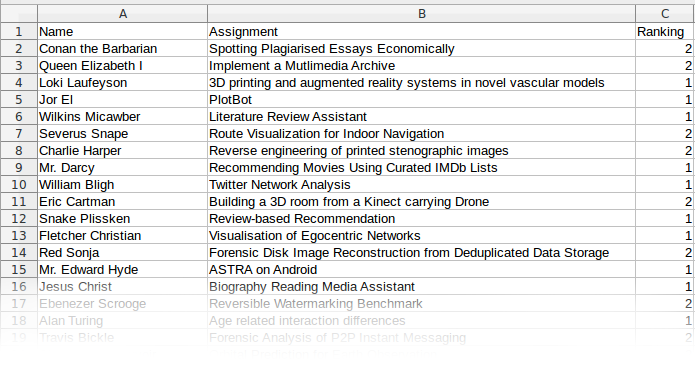
\includegraphics[width=0.92\columnwidth]{egout} % Example image
\end{center} 
\end{homeworkSection}
\newpage
\begin{homeworkSection}{The Graphical User Interface}
The simplicity and re-usability of our code was extremely important to us throughout this project, as discussed in our core values. To allow users to easily navigate their way through our software, regardless of its application, we created our Gui following these requirements. The Gui contains only three buttons - load a preference file, create a solution and save the created solution. Once the algorithm begins, a progress bar updates within the Gui to inform the user of the current status. This interface makes use of our hybrid solution - using simulated annealing to create the population for the genetic algorithm. This is discussed in further detail in Performance Analysis.%
\begin{center}
\textit{The Graphical User Interface}\\
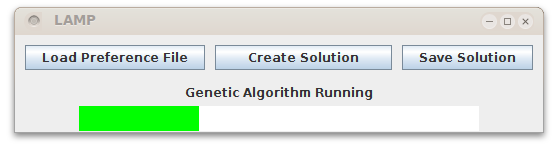
\includegraphics[width=0.7\columnwidth]{SimpleGui} % Example image
\end{center} 
\end{homeworkSection}
\begin{homeworkSection}{The Command Line Version}
This version of our software solution is for the advanced user. It gives the user the ability to specify which of the algorithms to run and under which parameters. These options are passed as command line arguments to the program, as well input and output file names. There is a help option which can be displayed with the "-help" tag.\\
The data used for performance analysis was created with the command line version of our program with the "-test" tag. This instructs the program to run each of the three algorithms (Simulated Annealing, Genetic and Hybrid) numerous times with varying parameters. The results of these tests are output to three separate tsv files.\\
To use the Cli, specify "-ga" for the genetic algorithm or "-sa" for the simulated annealing algorithm with the relevant parameters as specified below.
\begin{center}
\textit{The usage message}\\
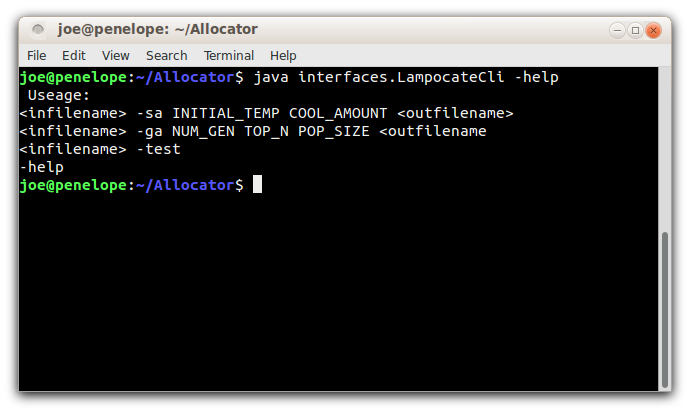
\includegraphics[width=0.85\columnwidth]{helpString}
\end{center}
\newpage

\textbf{Example program runs}\\
Note: Where the graphic user interface has a progress bar and text field for status updates, the Cli version of our solution uses the console. As the algorithm progresses, the sequence of dots grows in proportion with the algorithms progress and status updates are presented as lines of console output.\\
\begin{center}
\textit{The Cli used with the Genetic Algorithm}\\
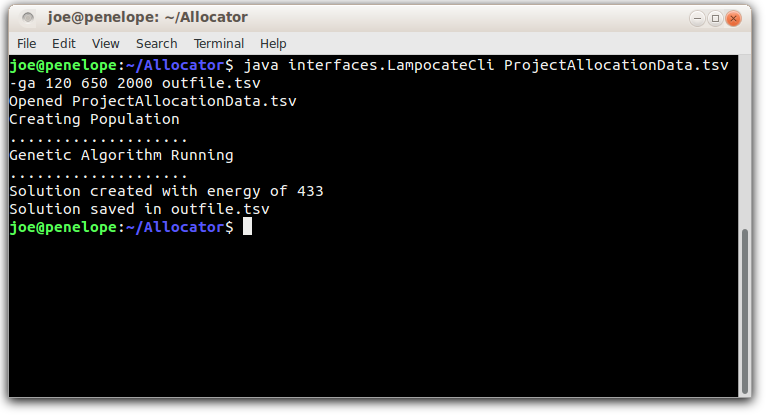
\includegraphics[width=0.95\columnwidth]{CliGa} % Example image
\end{center}
\vspace{0.6cm}
\begin{center}
\textit{The Cli used with the Simulated Annealing Algorithm}\\
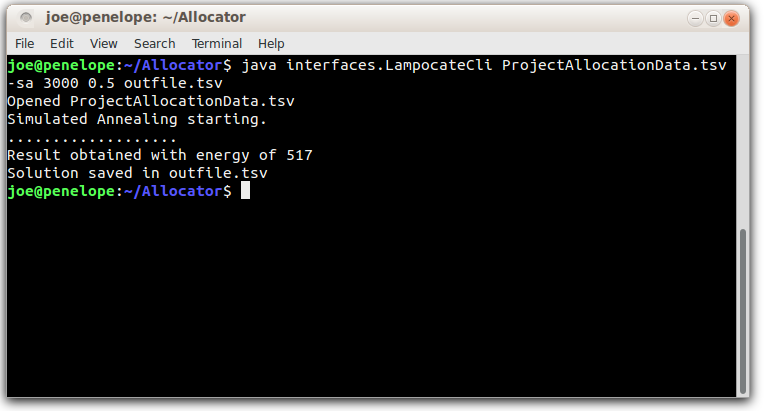
\includegraphics[width=0.95\columnwidth]{CliSa} % Example image
\end{center}
\end{homeworkSection}








\end{homeworkProblem}
\newpage

%---------------------------------------------------------------------------------------
\begin{homeworkProblem}[Class Diagrams]

In this section we present certain case specific arrangements of class diagrams. These demonstrate the modularity of our solution.

\begin{homeworkSection}{The Gui with Simulated Annealing and the Genetic Algorithm}
The Gui relies on the Link to get access to both the Simulated Annealing and Genetic Algorithms.  The 1 to 1 relationships between the CallBackListener and the algorithms allow the algorithms to update the status bar and text on the Gui.
\begin{center}
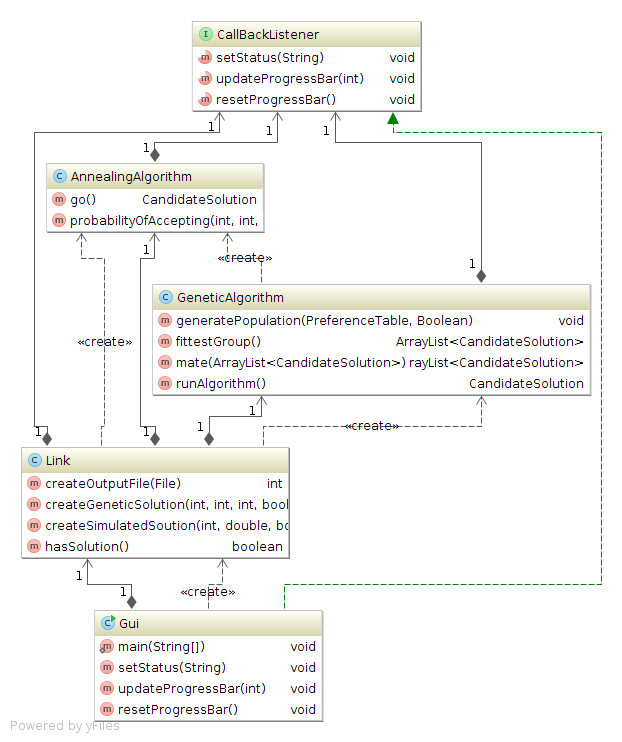
\includegraphics[width=0.99\columnwidth]{Gui} % Example image
\end{center}
\end{homeworkSection}
\newpage
\begin{homeworkSection}{Cli for Simulated Annealing}
The Cli has a 1 to 1 relationship with the Link, which is shown here to give access to the Simulated Annealing algorithm. This, in turn, has a 1 to 1 relationship with a Candidate Solution which it permutes. 
\vspace{0.4cm}
\begin{center}
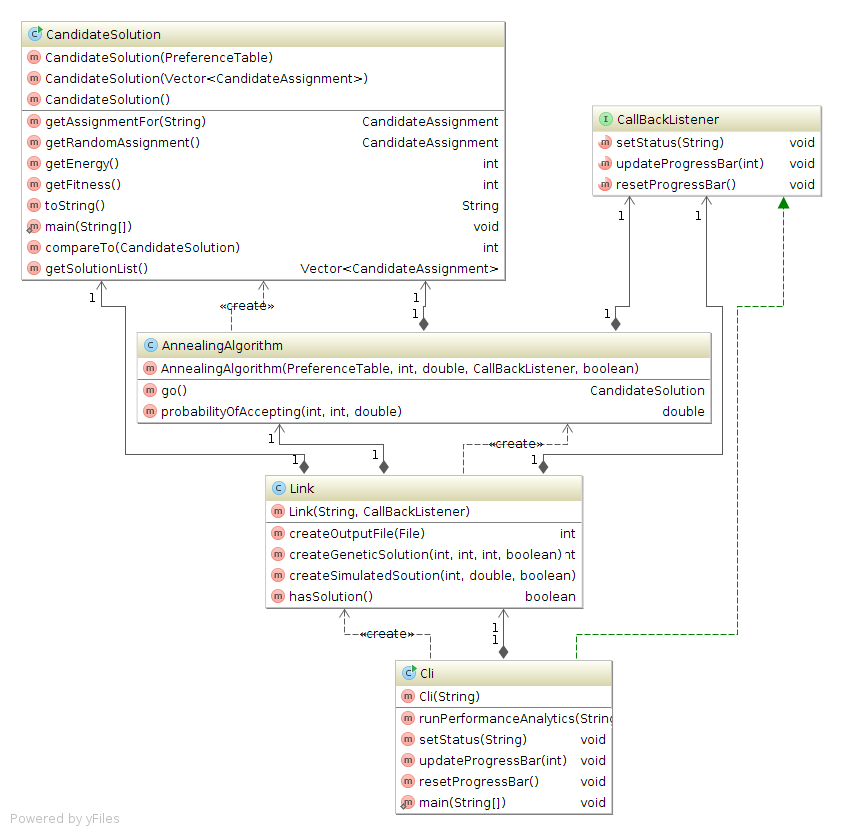
\includegraphics[width=0.99\columnwidth]{Cli-Annealing} % Example image
\end{center}
\end{homeworkSection}
\newpage
\begin{homeworkSection}{Cli for the Genetic Algorithm}
When the user elects to use the Genetic Algorithm, the 1 to 1 relationship between the Link and the Genetic Algorithm is used. In the diagrams below the inheritance relationship the ChildCandidateSolution and the CandidateSolution is evident.
\vspace{0.4cm}

\begin{center}
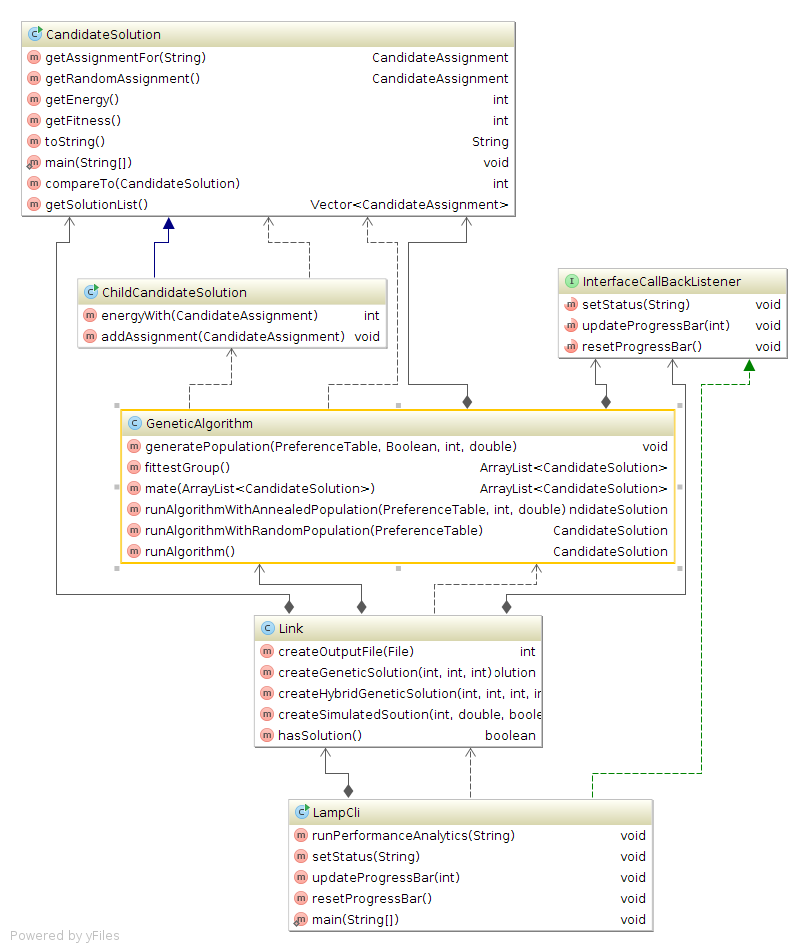
\includegraphics[width=0.99\columnwidth]{Cli-Genetic} % Example image
\end{center}
\end{homeworkSection}

\newpage
%------------------------------------------------------------------------------------------
\begin{homeworkProblem}[Performance Analysis]
Each algorithm has its own set of parameters which are needed and these have a significant effect on the overall energy of the given solution. We wanted our Gui to be a simple no frills program to give the ultimate solution so we removed the option of user input parameters. They are set as constant. In order to determine the best constants we ran overnight tests, subjecting each algorithm to a barrage of parameters. These results can be reproduced using the '-test' tag with in Cli version of our code. 
\\\\
If an advanced user wishes to specify their own parameters, the Cli version of our program will facilitate that.

\begin{homeworkSection}{The Genetic Alogrithm}
The Genetic Algorithm has 3 parameters:
\begin{itemize}
\item The initial population size
\item How may of the population to choose for mating (The top N)
\item The number of generations the population should evolve through
\end{itemize}
The overnight test yielded the following graph.

\begin{center}
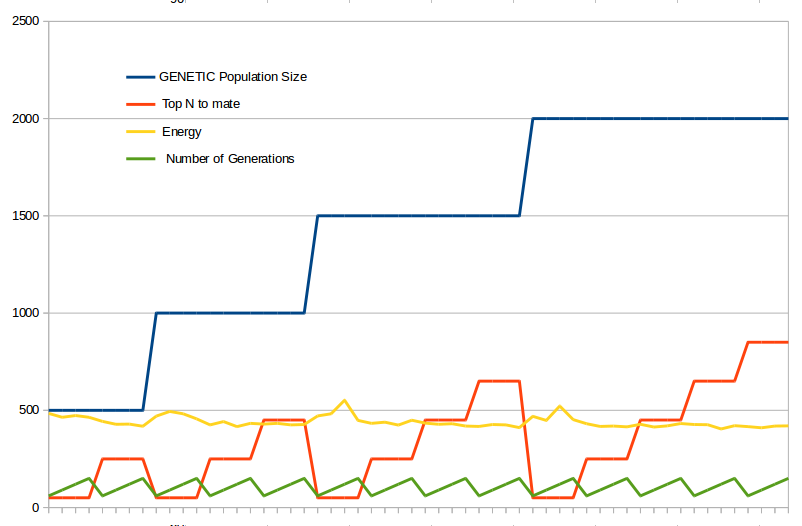
\includegraphics[width=0.9\columnwidth]{GaPerf} % Example image
\end{center}

The algorithm was ran with a variety of population sizes, number to mate and number of generations and the best parameters which gave the lowest energy were extracted.
\begin{description}
\item[Population Size:] 1500
\item[Top N:] 850
\item[Number of Generations:] 120
\end{description}

\end{homeworkSection}


\begin{homeworkSection}{The Simulated Annealing alogrithm}
The Simulated Annealing Algorithm has 2 parameters:
\begin{itemize}
\item The initial temperature of the solution
\item The amount the solution cools on each iteration.
\end{itemize}
The overnight test yielded the following graph.
\begin{center}
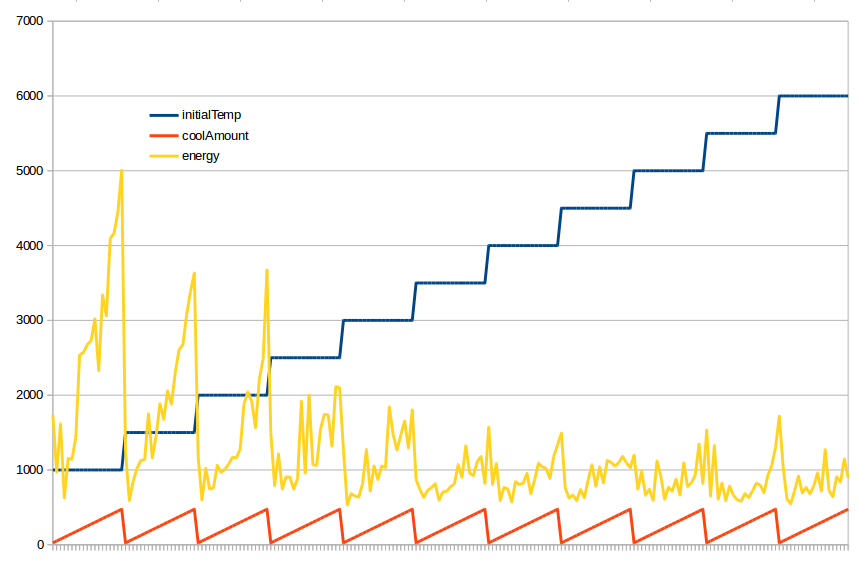
\includegraphics[width=0.9\columnwidth]{SaPerf} \\
\end{center}

The algorithm was ran with a variety of cooling amounts for a variety of initial temperatures. The cool amount has been scaled by a factor of 100 for clarity. The best parameters are shown below.
\begin{description}
\item[Initial Temperature] 3000
\item[Cooling Amount] 0.5
\end{description}

\end{homeworkSection}
\newpage
\begin{homeworkSection}{The Hybrid Algorithm}
The Hybrid Algorithm uses both algorithms to create a solution. The primary driver is the Genetic Algorithm but instead of a random initial random population, a population of solutions is created using simulated annealing.\\

The overnight test for this algorithm permuted over all 5 parameters:
\begin{itemize}
\item The initial population size
\item How may of the population to choose for mating (The top N)
\item The number of generations the population should evolve through
\item The initial temperature of the solution
\item The amount the solution cools on each iteration.
\end{itemize}
The overnight test yielded the following graph.
\begin{center}
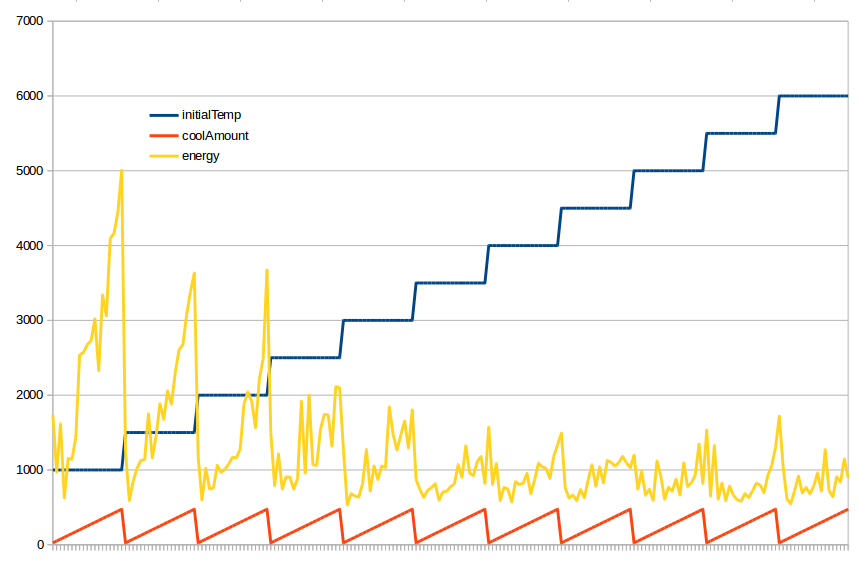
\includegraphics[width=0.9\columnwidth]{HyPerf} \\
\end{center}

The algorithm was ran with all permutations of the 5 parameters and we found these to produce the lowest energy. These are the parameters that we used in the Gui to attain the ultimate solution.
\begin{description}
\item[Population Size:] 2000
\item[Top N:] 650
\item[Number of Generations:] 120
\item[Initial Temperature] 3000
\item[Cooling Amount] 0.5
\end{description}

\end{homeworkSection}
\newpage
\begin{homeworkSection}{Comparing the Three Algorithms}

After attaining the optimal parameters for each algorithm we ran some scripted tests to get an average energy over 1000 iterations and produced the following graph.

\begin{center}
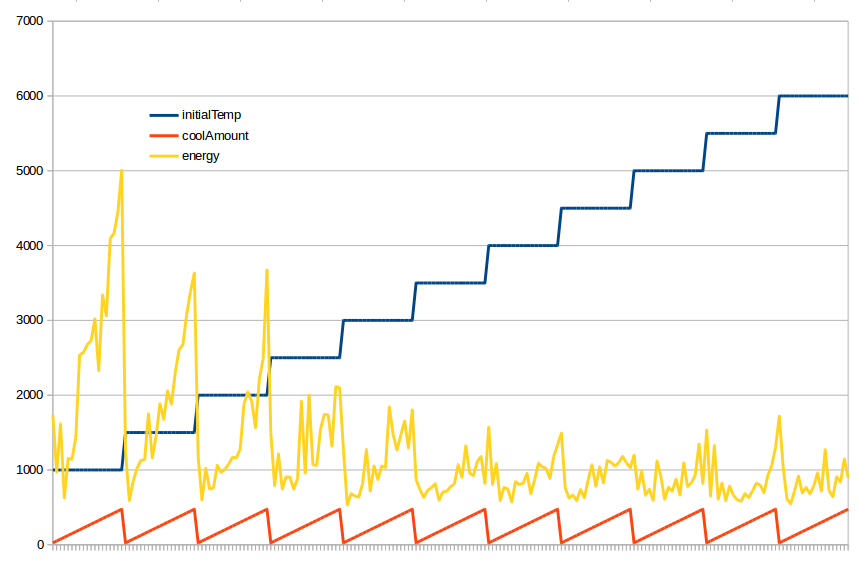
\includegraphics[width=0.9\columnwidth]{PerfComp} \\
\end{center}

\begin{description}
\item[Simulated Annealing] \ \\We used the optimal parameters defined above
\item[Genetic] \ \\ We used the optimal parameters defined above
\item[Hybrid Algorithm A] \ \\ We used the optimal parameters defined in the individual tests from above
\item[Hybrid Algorithm B] \ \\ We used the optimal parameters defined by the extensive testing of all the permutations of the 5 parameters.

\end{description}

This testing has defined the best set of parameters to use for our Gui.

\begin{description}
\item[Population Size:] 2000
\item[Top N:] 650
\item[Number of Generations:] 120
\item[Initial Temperature] 3000
\item[Cooling Amount] 0.5
\end{description}

\end{homeworkSection}



\end{homeworkProblem}
\newpage
%------------------------------------------------------------------------------------------
\begin{homeworkProblem}[Development Phases/Issues]
\vspace{.5cm}
\begin{homeworkSection} {The Design Pattern}
During our first meeting we discussed how our project would be organized, and the overall goals that we hoped to achieve. In keeping with our core values of modularity and re-usability we knew needed a solid design pattern to build upon.

Initially our first thought was that both the algorithms would inherit CandidateSolution and implement extra functionality as necessary. There would be a Gui at the front with instances of both algorithms. Further investigation into the requirements of the project led us see how the first implementation would cause too many road blocks. We settled on a linear design pattern with a very directed data flow from the interface to the link to the algorithm. This is discussed further in the technical details section.\\

\begin{center}
\textit{The old and new design patterns}\\
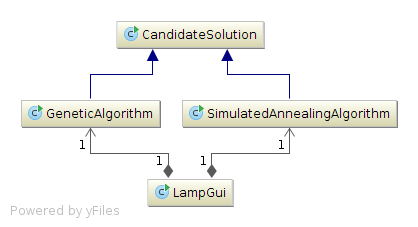
\includegraphics[width=0.45\columnwidth]{crapDesign} 
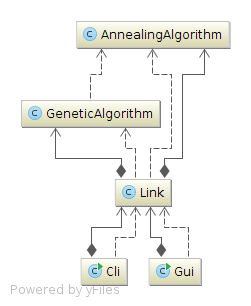
\includegraphics[width=0.27\columnwidth]{DesignPattern} % Example image

\end{center}

\begin{center}
\end{center}


With the overall picture in our heads of the direction we were going we began development the 2 algorithms, the link and the interfaces, with each of us being assigned a particular section.\\

\end{homeworkSection}

\newpage
\begin{homeworkSection}{The Genetic Algorithm}
\begin{description}

\item[The initial setup]\ 

For the genetic algorithm, generations are the key to improving a solution. There were three main steps to consider. Generating a population, mating the best candidates, and replacing the weakest members of the population with the children created from the mating process. This finalized group would then become the population for the next generation.
The idea is that each generation will become stronger and yield a good result.

A good result in the scope of our program would be considered one with minimal energy. Energy was chosen as a marker for consistency throughout the program with both the genetic and annealing algorithm referring to it. 

\item[Creating the population]\ 

Creating a population was a relatively easy step due to the strong framework which we already had in place and which was discussed in our interim report. 

generatePopulation is the function which we designed to create an ArrayList of randomly selected CandidateSoltions. Using this type of data structure allowed us to easily amend our population by sorting it and adding/removing members which will become important once the algorithm has run. 

This strong basis meant that this function remained consistent throughout the development process and changed very little from beginning to end.

\item[Finding the fittest group]\ 

In order for our solution to improve in each generation, we needed to find the best members of the population (or the members which have the lowest energy scores). The Collections class allowed us to compare each member of the population based on their energy simply by implementing a compareTo method within the CandidateAssignment class. Once the population was sorted on this criteria it was simply a matter of selecting the top N elements of the population, with N being an even number, the size of which we would like our fittest group to be. Initially these were set as constants for ease of testing.


\item[Finding the weakest group]\ 

With the population already sorted, finding the weakest group was trivial, and ArrayList contained all of the tools necessary for removing the lowest elements and adding in the children created during the mating process.


\item[Mating]\ 

Mating was the most complex element of this algorithm and as such was subject to a lot of change throughout the development cycle. Firstly we needed to decide what mating actually meant for this program and how it would ultimately improve the solution. 

As a group we discussed the different elements. Taking into account the project specifications and what we ultimately wanted to achieve. We came to the conclusion that the mating should happen on the level of CandidateAssignments as this is where the energy really originates. 

\item[First run]\ 

Each member  of the fittestGroup was paired with their neighbor in the array. This meant that best solutions stayed with the best solutions. The idea being that these would in turn result in the best children. 

Our algorithm took the two parents, both of whom are CandidateSolutions, and created a new CandidateSolution child based on the best elements of these parents. The CandidateAssignments within the parents are always listed in order. This meant that we could iterate through the parents and compare each Candidate assignment. 

Additional code was added to the CandidateAssignment class which would allow us access to each students satisfaction. Whichever student had the better satisfaction score was then used in creating the child. This meant that the child was essentially a combination of the most satisfied students. 

\item[Results]\ 

This process resulted in a relatively poor score and two large obstacles became apparent. 

A large penalty is applied whenever there is a duplication in project selections among students.  Our algorithm did not take into account a project allocation already existing within the child solution. So, while the solution was better for the individual student, The overall energy produced by the solution incurred a huge penalty.

The other big problem which occurred was that as our list of fittest solutions was sorted every generation, often the same parents would produce identical children each generation. This meant that our solution became full of duplicates and stopped improving after only a few generations.


\item[Revising the approach]\ 

While the overall approach to mating was sound, our implementation was flawed.  These situations needed to be handled. 

The algorithm was restructured completely while retaining the core ideas. The individual Candidate assignments were still compared but other checks were applied. 

We introduced a ChildCandidateSolution class with the function energyWith(). This allowed us to check whether the overall energy would improve, preventing larger penalties from incurring. 


To prevent the possibility of identical parents producing an identical child, the fittest group was shuffled and a new check was introduced. Before each child can be added to the children list, its energy must be greater than the energy of both parent1 and parent2. 
All of the children who don’t make the cut are drowned in a river and discarded. 


\item[Results]\ 

Immediately results were much better. With energy dropping from the thousands into the range of 300-400

\item[Mutations]\ 

An element of the Genetic algorithm is the idea of mutations. A mutation is a random adjustment made in some way to the solution. 

We initially introduced a random student assignment (with adjustable mutation frequency) and moved this onto a random candidate assignment added into the population. 

After running numerous tests with both of these possibilities, and various mutation frequencies, we discovered that no improvement to the final solution was made. In fact, the solution often fluctuated resulting in poorer final results.

After discussing the possibilities we decided as a group to remove mutation entirely. While it is an interesting element of the genetic algorithm, it took us further from our goal of achieving a good low energy score.

\end{description}

\end{homeworkSection}

\begin{homeworkSection}{The Simulated Annealing Algorithm}

With the annealing algorithm, we searched for an overall optimum solution as opposed to an actual best solution, we wanted to consider time as a factor. The three main areas for development were the temperature, the cooling amount, the probability of accepting a solution and the algorithm that drives everything. \\

\begin{description}

\item[Approach]\ 

The class was first written entirely in pseudo code, which allowed for any logical obstacles to be addressed and overcome before implementing any code. Helper methods were created as required by the pseudo code, with the possibility of these being added to or removed as the program functionality was tested.

\item[The Boltzmann Formula]\ 

The algorithm was then written in full. The Boltzmann formula was used to help us find our solution. Annealing works similar to a hill climbing search, however once a local max is found, there is a possibility to keep searching and to find an even greater result. To calculate the probability of the change in solution being accepted, we created a separate method to include the Boltzmann distribution value for the energy and temperature of a certain solution.

\begin{center}
\textit{The Boltzmann Formula}\\
$p(\bigtriangleup E) = \frac{1}{e^{\frac{\bigtriangleup E}{T}}}$
\end{center}

\item[Parameters]\ 

It is here that the Temperature and cooling come into play. The temperature is set and applied to the algorithm, the higher the temperature then the looser the algorithm and the more likely that a bad solution is accepted. The cooling amount is applied to the temperature meaning we are less and less likely to accept a poor answer. 

\item[Refinements with Inlining]\ 

We initially created a helper method to randomize an element of the solution. Keeping in line with our original ethos and attempting to maintain a good flow with readable code, this evolved to be a very small method. The choice was made to included it in our go method instead.  The notion of a ‘go’ method, meant that while looking through the code, it was easy for any user to track what was happening should any revisions need to be made. 

\item[Final Refinements]\ 

The program initially had constant values for temperature and the amount to be cooled by each time. In testing this, these were altered to determine what combination of variables achieved the best results in under a minutes computation time. This was then altered to allow the user to enter these values as desired through the CLI.\\

After this was finished, we merely added in functionality to alter the progress bar and allow for status updates as the algorithm begins and ends, before cleaning up the flow of the code and ensuring all variables were global/private as required.

\end{description}
\end{homeworkSection}

\begin{homeworkSection}{The Interfaces} 
The first aim of the first Gui was to provide all the functionality of our algorithms. We implemented it with the swing packages and produced a very functional piece of software. After really thinking about the goal of this project we decided this was too much. We wanted to produce an easy to use solution with optimal parameters that were preset and decided upon through thorough testing.
\\
\begin{center}
\textit{The old and complicated Gui}
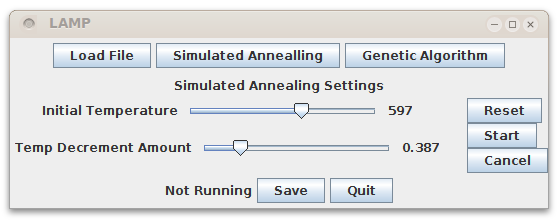
\includegraphics[width=0.76\columnwidth]{ComplexGui} % Example image
\end{center}
\vspace{0.5cm}
The realisation of a need for a simple Gui opened the option of a much more functional command line versions of our software. Initially we produced two different interfaces, one for each algorithm. These were beneficial for testing but were ultimately combined into a comprehensive Cli which compliments our user friendly Gui.

\end{homeworkSection}{}
\vspace{0.5cm}
\begin{homeworkSection}{Development Cycle Conclusion}
One of our mission statements was to create clean, readable code. Once we finished the main coding and testing, we then proceeded to run through the code, being extra critical about its ordering and functionality. 

The names of the functions were refactored to reflect the modularity of those functions. Encapsulation was refined to ensure elements were public only if required. 

More parameters were added to constructors in order to allow adjustments and commands to be input through the CLI and GUI.  
\end{homeworkSection}






\end{homeworkProblem}
\newpage

%---------------------------------------------------------------------------------------
\begin{homeworkProblem}[Our Development Model]



\begin{homeworkSection}{Not sure what needs to go in here}

\end{homeworkSection}






\end{homeworkProblem}
\newpage

%---------------------------------------------------------------------------------------
\begin{homeworkProblem}[Technical Details Of Note]


\begin{homeworkSection}{Our Design Pattern}
In keeping with our core values of simplicity and re-usability we tried to use a very modular design pattern. We identified two distinct types of classes that we created, worker classes and interfaces (the algorithms and the Cli/Gui respectively). An interface invokes methods on a worker. In order to modularise this we created a Link class. This is a pivotal class in our design. Every method call from an interface must go through the link. This gives the ability to pair any interface with any algorithm with ease. Once an interface has access to a Link it can call upon either or both of the algorithms as is necessary. The linear flow of our design pattern is very evident below.
\begin{center}
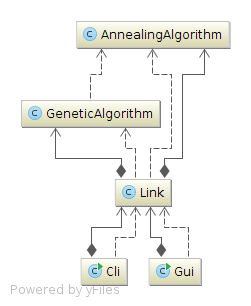
\includegraphics[width=0.27\columnwidth]{DesignPattern} % Example image
\end{center}
\end{homeworkSection}


\begin{homeworkSection}{Callback listeners}
Independent communication between classes is typically one directional. Usually a class invokes a method on one of the classes that it has references to and a single value is returned upon completion. Sometimes the need for interaction with the calling class is needed during execution of the called method; this is where callback listeners come in. They provide the ability for a method to invoke a method on the calling class.\\\\
Use of callback listeners:
\begin{enumerate}
\item The listener is ultimately an interface. It declares which methods in the calling class are available to class containing the called method.
\item The calling class implements each of the methods declared in this interface.
\item When creating an instance of a class, whose methods will be called at some point, a reference to the calling class is passed using the "this" keyword to the classes constructor.
\item That class, which needs the reverse communication path, then instantiates an object of type callback listener with the passed reference. 
\item This allows method calls back to the calling class during execution and also keeps encapsulation tight as it does not provide the full public interface of the calling class.
\item Callback listeners can also be used with threads to alert the class which created the thread of completion or another significant event.
\end{enumerate}
In our project methods in the algorithm classes are invoked by either of the interface classes (via the Link). We used a callback listener to allow both the Genetic and Simulated Annealing algorithms to invoke methods on which ever interface invoked the algorithm. The callback listener is a direct connection straight back to the calling class. 
\\We used the listener to update the progress bar every time 10 percent of the total number of iterations have been completed and also when the status bar needed updating with new information. Our two interfaces, the Cli and Gui, both implement the callback listener and have their own respective versions of the status bar and progress bar.

\end{homeworkSection}
\begin{homeworkSection}{Inheritance}
When building software, in order to efficiently utilise the classes at one's disposal. it is always important to be mindful of potential inheritance relationships. An inheritance relationship gives a subclass access to the methods and fields of the superclass. Inheritance is used when needing to add case specific functionality to a class, i.e. extra functionality that would otherwise bloat other clients of the class. 
\\\\
We identified a need to subclass the CandidateSolution class when creating the Genetic Algorithm. The Genetic Algorithm has to build a CandidateSolution one project at a time and also query the potential fitness of that solution during the building phase. This led to the creation of the ChildCandidateSolution class, which inherits from CandidateSolution, with two extra methods, evident below.
\begin{center}
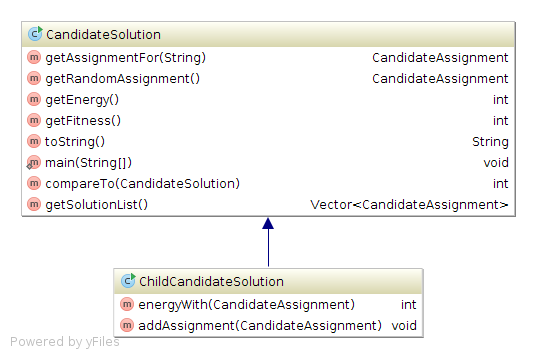
\includegraphics[width=0.60\columnwidth]{Inheritance} % Example image
\end{center}

\end{homeworkSection}

\begin{homeworkSection}{Threads} 
By default programs run on one main thread. They have one time line, one stream of execution, on which the programs instructions are carried out consecutively. Sometimes, when expensive routines are needed to be called it's advantageous to put them on their own thread, their stream of execution. When the routine is complete is typically not known, but it will complete at some point, (assuming no runtime/logic errors). Callback listeners can be used to signal the main thread of completion or some other significant event. 
\\\\
In our project, the Cli runs in only one thread, and procedurally runs the algorithm and prints the the console to indicate its progress. During execution the user has no interactivity with the program as it's main thread is blocked by the expensive task of computing a solution.\\
When we designed the Gui it became evident that a separate execution thread was needed as there are two tasks to complete. The Jframe that is the Gui needs redrawing with the progress bar updates and the algorithm has to be executed. We created a separate thread on which the algorithm would run, allowing these two tasks to done concurrently.
\end{homeworkSection}{}







\end{homeworkProblem}
\newpage

%---------------------------------------------------------------------------------------

\begin{homeworkProblem}[Team Development]

what we changed\\
what we liked/didnt,\\
stuckto/deviated from interim\\

\begin{homeworkSection}{What went well}
the night out and the burgers

\end{homeworkSection}

\begin{homeworkSection}{What didn't go so well}
everything else
\end{homeworkSection}


\begin{homeworkSection}{Who did what}
everything else
\end{homeworkSection}{}


\end{homeworkProblem}



\newpage









\end{homeworkProblem}
\newpage

%---------------------------------------------------------------------------------------

\begin{homeworkProblem}[The Team Night Out]
\begin{homeworkSection}{Burgers and Drama}
The development of a large software project involves both individual and group contributions. Many large tasks were broken up into smaller subsections which were divided between the team members. These were researched and brainstormed individually before meeting as a group and developing solutions together. 

To keep morale high while we worked through the assignment, we organized a team bonding night between the interim report and the submission of the final report. This took place after a long group coding session in college where the bones of both algorithms were written. We felt that an evening of discussion on topics other than the software project would help keep us connected as a group, which would improve overall work ethic and quality of code produced.

The team night out involved travelling together into town for a large dinner, before returning to UCD campus for a production of The Nightman Cometh (an episode of the popular TV show It's Always Sunny in Philadelphia) by UCD's DramaSoc. A night off from code development and report writing was well deserved and earned, and allowed for the team to work harder upon our return to college the next day.
\end{homeworkSection}
\end{homeworkProblem}

%----------------------------------------------------------------------------------------
\begin{homeworkProblem}[A Sad Day For Lamp]

\begin{homeworkSection}{The loss of a team member}
As a young adult, college can often be a very stressful and time consuming environment to be in. A large amount of students are dropping out of all courses, with 23\% of students entering the computer science program in UCD not progressing past their first year. Unfortunately for Team Lamp, we experienced a loss of a member partway through the development process.

Team Lamp started off well, producing strong weekly assignments by each team member. Sadly, we found that as time passed, one member was slowly fading off the radar and was no longer contributing towards the module in both individual assessments and team projects. Gerard Fogarty, our lost Lamp, has unfortunately not been a presence within the team for several weeks. 

Team Lamp has persevered through this loss, providing what we feel is still a marketable software solution to this module's brief. Although this module heavily suggested teams of four to produce a solid working solution, we feel that we overcame the obstacle of having only three team members and still maintained a high quality software project and solid written report. 
\\
\end{homeworkSection}
\begin{center}
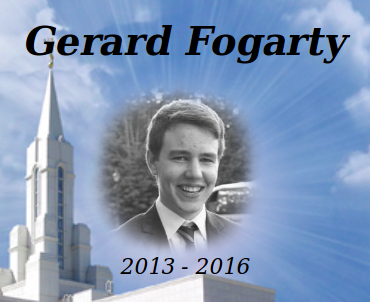
\includegraphics[width=0.46\columnwidth]{obituary} % Example image
\end{center}
\end{homeworkProblem}
\end{document}
\newpage
%----------------------------------------------------------------------------------------
\begin{homeworkProblem}[Conclusion]
\begin{homeworkSection}{The loss of a team member}
We suffered a tragic loss,,, Gerard has become a lost lamp
\end{homeworkSection}
\end{homeworkProblem}
\end{document}